%%%%%%%%%%%%%%%%%%%%%%%%%%%%%%%%%%%%%%%%%%%%%%%%%%%%
%\graphicspath{chapters/figures/}
\section{Write Back}
\label{chap_wb}

%%%%%%%%%%%%%%%%%%%%%%%%%%%%%%%%%%%%%%%%%%%%%%%%%%%%%%%%%%%

The \textit{Write Back} stage is needed to write in the registers the final result obtained after the execution and the access to memory. With this goal, an destination address is needed, as well as some muxes to select the right signal to be sent back to the \textsf{RF}. The overall structure is presented in figure \ref{wb_overall_fig}.
Few signals are needed in the entire unit:
\begin{itemize}
	\item \textbf{MEM\_ALU\_SEL}, selection signal coming from the control word, controlling the output mux
	\item \textbf{DEST\_IN}, destination address from the memory stage
	\item \textbf{FROM\_ALU}, coming directly from the execution stage
	\item \textbf{FROM\_MEM}, that comes from the memory, after a read operation has been performed
	\item \textbf{DATA\_OUT}, which contains the data to be written on the 
	\textsf{RF}
	\item \textbf{DEST\_OUT}, destination address to the \textsf{RF}
\end{itemize}

\begin{figure}
	\centering
	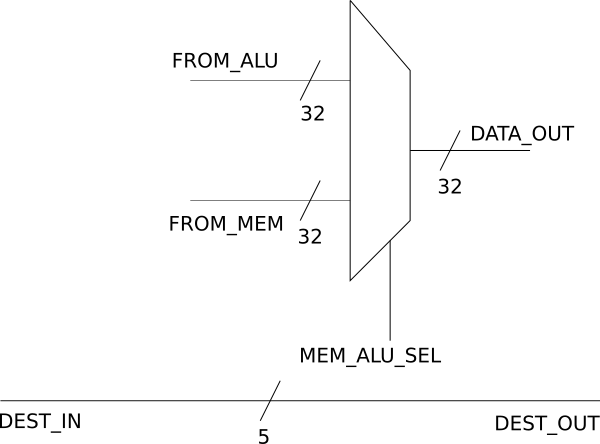
\includegraphics[scale=0.5]{chapters/figures/wb_stage}
	\caption{Mux to choose the required output}
	\label{wb_overall_fig}
\end{figure} 

To simply explain the behavior, one can say that the destination address is 
contained in the 5 bits of \textit{DEST\_IN}, which are passed to 
\textit{DEST\_OUT}. This output signal is then connected to the \textsc{RF}, 
where the \textit{WR} signal enables the writing. The actual value that is 
written on memory is chosen between the outputs from memory and ALU, and 
ultimately written to close the pipeline and complete the instruction, which is 
finally committed at the start of the next cycle.




